\documentclass[12pt,a4paper]{report}
\usepackage{cclicenses}
\usepackage{graphicx}
\title{Ceph Training Materials}
\author{Victor Denisov}
\date{\today}
\begin{document}
   \maketitle
\begin{abstract}
This work, ``Ceph Training Materials'', is derivative of ``Ceph Documentation'' http://docs.ceph.com/docs/master/ by Victor Denisov, used under \bysa. ``Ceph Documentation'' is licensed under \bysa by Inktank.
\end{abstract}

% Makes emph bold by default.
\makeatletter
\DeclareRobustCommand{\em}{%
  \@nomath\em \if b\expandafter\@car\f@series\@nil
  \normalfont \else \bfseries \fi}
\makeatother

\chapter{Ceph Architecture}
Ceph uniquely delivers object, block, and file storage in one unified system.
A Ceph Node leverages commodity hardware and intelligent daemons, and a Ceph
Storage Cluster accommodates large numbers of nodes, which communicate with
each other to replicate and redistribute data dynamically. All the components
of ceph storage cluster are presented on figure \ref{fig:ceph_architecture}

\begin{figure}[h]
	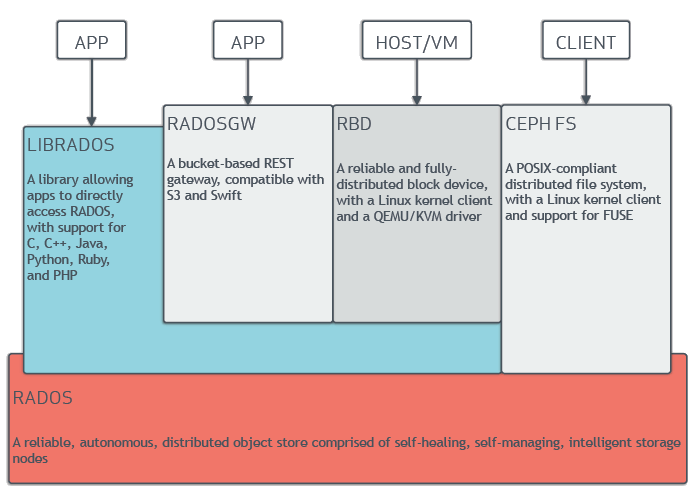
\includegraphics[scale=0.5]{stack.png}
	\caption{Ceph Architecture}
	\label{fig:ceph_architecture}
\end{figure}

\section{The Ceph Storage Cluster}
Ceph provides an infinitely scalable Ceph Storage Cluster based upon RADOS.
RADOS means Reliable Autonomic Distributed Object Store.

A Ceph Storage Cluster consists of two types of daemons:

\begin{itemize}
	\item Ceph Monitor
	\item Ceph OSD Daemon
\end{itemize}

A Ceph Monitor maintains a master copy of the cluster map. A cluster of Ceph
monitors ensures high availability should a monitor daemon fail. Storage
cluster clients retrieve a copy of the cluster map from the Ceph Monitor.

A Ceph OSD Daemon checks its own state and the state of other OSDs and reports
back to monitors.

Storage cluster clients and each Ceph OSD Daemon use the CRUSH algorithm to
efficiently compute information about data location, instead of having to
depend on a central lookup table. Ceph’s high-level features include providing
a native interface to the Ceph Storage Cluster via librados, and a number of
service interfaces built on top of librados.

\subsection{Storing Data}

The Ceph Storage Cluster receives data from Ceph Clients–whether it comes
through a Ceph Block Device, Ceph Object Storage, the Ceph Filesystem or a
custom implementation you create using librados–and it stores the data as
objects. Each object corresponds to a file in a filesystem, which is stored on
an Object Storage Device. Ceph OSD Daemons handle the read/write operations on
the storage disks.

\begin{figure}[h]
	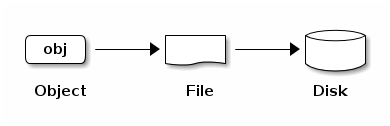
\includegraphics[scale=0.75]{object_file_disk.png}
	\label{fig:object_file_disk}
\end{figure}

Ceph OSD Daemons store all data as objects in a flat namespace (e.g., no
hierarchy of directories). An object has an identifier, binary data, and
metadata consisting of a set of name/value pairs. The semantics are completely
up to Ceph Clients. For example, CephFS uses metadata(figure
\ref{fig:object_metadata}) to store file attributes such as the file owner,
created date, last modified date, and so forth. \emph{Every object has an id which is
unique across the entire ceph cluster, not just the local filesystem.}

\begin{figure}[h]
	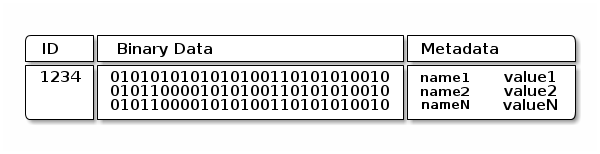
\includegraphics[scale=0.60]{object_metadata.png}
	\caption{Object's Metadata}
	\label{fig:object_metadata}
\end{figure}

\subsection{Scalability and High Availability} \label{scal_and_high_avail}

In traditional architectures, clients talk to a centralized component (e.g., a
gateway, broker, API, facade, etc.), which acts as a single point of entry to a
complex subsystem. This imposes a limit to both performance and scalability,
while introducing a single point of failure (i.e., if the centralized component
goes down, the whole system goes down, too).

Ceph eliminates the centralized gateway to enable clients to interact with Ceph
OSD Daemons directly. Ceph OSD Daemons create object replicas on other Ceph
Nodes to ensure data safety and high availability. Ceph also uses a cluster of
monitors to ensure high availability. To eliminate centralization, Ceph uses an
algorithm called CRUSH.

\subsection{CRUSH Introduction}

Ceph Clients and Ceph OSD Daemons both use the CRUSH algorithm to efficiently
compute information about object location, instead of having to depend on a
central lookup table. CRUSH provides a better data management mechanism
compared to older approaches, and enables massive scale by cleanly distributing
the work to all the clients and OSD daemons in the cluster. CRUSH uses
intelligent data replication to ensure resiliency, which is better suited to
hyper-scale storage. The following sections provide additional details on how
CRUSH works. For a detailed discussion of CRUSH, see CRUSH - Controlled,
Scalable, Decentralized Placement of Replicated Data. \ref{crush_chapter}

\subsection{Cluster Map} \label{cluster_map}

Ceph depends upon Ceph Clients and Ceph OSD Daemons having knowledge of the
cluster topology, which is inclusive of 5 maps collectively referred to as the
``Cluster Map'':
\begin{enumerate}
	\item \emph{The Monitor Map}: Contains the cluster fsid, the position,
		name address and port of each monitor. It also indicates the
		current epoch, when the map was created, and the last time it
		changed. To view a monitor map, execute \emph{ceph mon dump}.
	\item \emph{The OSD Map}: Contains the cluster fsid, when the map was
		created and last modified, a list of pools, replica sizes, PG
		numbers, a list of OSDs and their status (e.g., up, in). To
		view an OSD map, execute \emph{ceph osd dump}.
	\item \emph{The PG Map}: Contains the PG version, its time stamp, the
		last OSD map epoch, the full ratios, and details on each
		placement group such as the PG ID, the Up Set, the Acting Set,
		the state of the PG (e.g., active + clean), and data usage
		statistics for each pool.
	\item \emph{The CRUSH Map}: Contains a list of storage devices, the
		failure domain hierarchy (e.g., device, host, rack, row, room,
		etc.), and rules for traversing the hierarchy when storing
		data. To view a CRUSH map, execute \emph{ceph osd getcrushmap -o
		filename;} then, decompile it by executing \emph{crushtool -d
		comp-crushmap-filename -o decomp-crushmap-filename}. You can
		view the decompiled map in a text editor or with cat.
	\item \emph{The MDS Map}: Contains the current MDS map epoch, when the
		map was created, and the last time it changed. It also contains
		the pool for storing metadata, a list of metadata servers, and
		which metadata servers are up and in. To view an MDS map,
		execute \emph{ceph mds dump}.
\end{enumerate}

Each map maintains an iterative history of its operating state changes. Ceph
Monitors maintain a master copy of the cluster map including the cluster
members, state, changes, and the overall health of the Ceph Storage Cluster.

\subsection{High Availability Monitors}

Before Ceph Clients can read or write data, they must contact a Ceph Monitor to
obtain the most recent copy of the cluster map. A Ceph Storage Cluster can
operate with a single monitor; however, this introduces a single point of
failure (i.e., if the monitor goes down, Ceph Clients cannot read or write
data).

For added reliability and fault tolerance, Ceph supports a cluster of monitors.
In a cluster of monitors, latency and other faults can cause one or more
monitors to fall behind the current state of the cluster. For this reason, Ceph
must have agreement among various monitor instances regarding the state of the
cluster. Ceph always uses a majority of monitors (e.g., 1, 2:3, 3:5, 4:6, etc.)
and the Paxos algorithm to establish a consensus among the monitors about the
current state of the cluster.

\subsection{High Availability Authentication}
To identify users and protect against man-in-the-middle attacks, Ceph provides
its cephx authentication system to authenticate users and daemons.  \emph{The
cephx protocol does not address data encryption in transport (e.g., SSL/TLS) or
encryption at rest.}

Cephx uses shared secret keys for authentication, meaning both the client and
the monitor cluster have a copy of the client’s secret key. The authentication
protocol is such that both parties are able to prove to each other they have a
copy of the key without actually revealing it. This provides mutual
authentication, which means the cluster is sure the user possesses the secret
key, and the user is sure that the cluster has a copy of the secret key.

A key scalability feature of Ceph is to avoid a centralized interface to the
Ceph object store, which means that Ceph clients must be able to interact with
OSDs directly. To protect data, Ceph provides its cephx authentication system,
which authenticates users operating Ceph clients. The cephx protocol operates
in a manner with behavior similar to Kerberos.

A user/actor invokes a Ceph client to contact a monitor. Unlike Kerberos, each
monitor can authenticate users and distribute keys, so there is no single point
of failure or bottleneck when using cephx. The monitor returns an
authentication data structure similar to a Kerberos ticket that contains a
session key for use in obtaining Ceph services. This session key is itself
encrypted with the user’s permanent secret key, so that only the user can
request services from the Ceph monitor(s). The client then uses the session key
to request its desired services from the monitor, and the monitor provides the
client with a ticket that will authenticate the client to the OSDs that
actually handle data. Ceph monitors and OSDs share a secret, so the client can
use the ticket provided by the monitor with any OSD or metadata server in the
cluster. Like Kerberos, cephx tickets expire, so an attacker cannot use an
expired ticket or session key obtained surreptitiously. This form of
authentication will prevent attackers with access to the communications medium
from either creating bogus messages under another user’s identity or altering
another user’s legitimate messages, as long as the user’s secret key is not
divulged before it expires.

To use cephx, an administrator must set up users first. In the following
diagram, the client.admin user invokes ceph auth get-or-create-key from the
command line to generate a username and secret key. Ceph’s auth subsystem
generates the username and key, stores a copy with the monitor(s) and transmits
the user’s secret back to the client.admin user. This means that the client and
the monitor share a secret key.

\emph{The client.admin user must provide the user ID and secret key to the user in a
secure manner.}

\begin{figure}[h]
	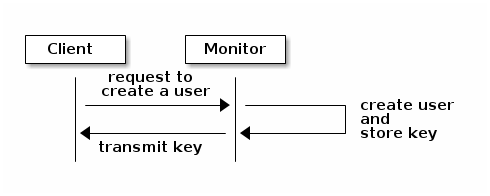
\includegraphics[scale=0.75]{create_user.png}
	\caption{User Creation}
	\label{fig:create_user}
\end{figure}

To authenticate with the monitor, the client passes in the user name to the
monitor, and the monitor generates a session key and encrypts it with the
secret key associated to the user name. Then, the monitor transmits the
encrypted ticket back to the client. The client then decrypts the payload with
the shared secret key to retrieve the session key. The session key identifies
the user for the current session. The client then requests a ticket on behalf
of the user signed by the session key. The monitor generates a ticket, encrypts
it with the user’s secret key and transmits it back to the client. The client
decrypts the ticket and uses it to sign requests to OSDs and metadata servers
throughout the cluster.

\begin{figure}[h]
	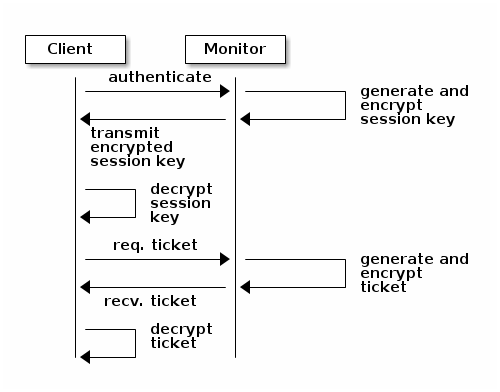
\includegraphics[scale=0.75]{ticket_retrieval.png}
	\caption{Ticket Retrieval}
	\label{fig:ticket_retrieval}
\end{figure}

The cephx protocol authenticates ongoing communications between the client
machine and the Ceph servers. Each message sent between a client and server,
subsequent to the initial authentication, is signed using a ticket that the
monitors, OSDs and metadata servers can verify with their shared secret.

\begin{figure}[h]
	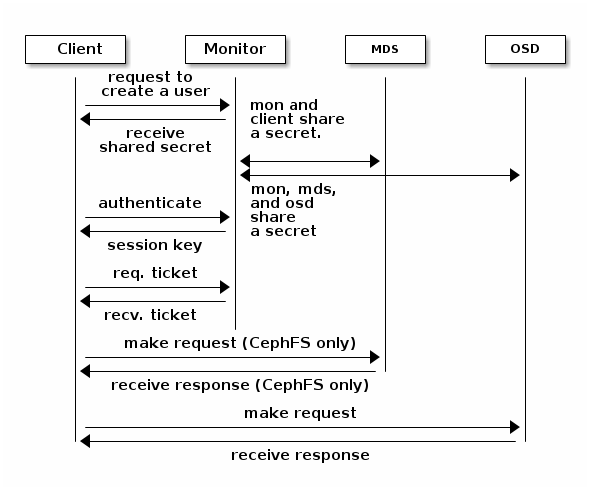
\includegraphics[scale=0.60]{request_to_osd.png}
	\caption{Secret Verification}
	\label{fig:ticket_retrieval}
\end{figure}

The protection offered by this authentication is between the Ceph client and
the Ceph server hosts. The authentication is not extended beyond the Ceph
client. If the user accesses the Ceph client from a remote host, Ceph
authentication is not applied to the connection between the user’s host and the
client host.

\subsection{Smart Daemons Enable Hyperscale}

In many clustered architectures, the primary purpose of cluster membership is
so that a centralized interface knows which nodes it can access. Then the
centralized interface provides services to the client through a double
dispatch–which is a huge bottleneck at the petabyte-to-exabyte scale.

Ceph eliminates the bottleneck: Ceph’s OSD Daemons AND Ceph Clients are cluster
aware. Like Ceph clients, each Ceph OSD Daemon knows about other Ceph OSD
Daemons in the cluster. This enables Ceph OSD Daemons to interact directly with
other Ceph OSD Daemons and Ceph monitors. Additionally, it enables Ceph Clients
to interact directly with Ceph OSD Daemons.

The ability of Ceph Clients, Ceph Monitors and Ceph OSD Daemons to interact
with each other means that Ceph OSD Daemons can utilize the CPU and RAM of the
Ceph nodes to easily perform tasks that would bog down a centralized server.
The ability to leverage this computing power leads to several major benefits:

\begin{enumerate}
	\item \emph{OSDs Service Clients Directly}: Since any network device
		has a limit to the number of concurrent connections it can
		support, a centralized system has a low physical limit at high
		scales. By enabling Ceph Clients to contact Ceph OSD Daemons
		directly, Ceph increases both performance and total system
		capacity simultaneously, while removing a single point of
		failure. Ceph Clients can maintain a session when they need to,
		and with a particular Ceph OSD Daemon instead of a centralized
		server.

	\item \emph{OSD Membership and Status}: Ceph OSD Daemons join a cluster and
		report on their status. At the lowest level, the Ceph OSD Daemon status
		is up or down reflecting whether or not it is running and able to
		service Ceph Client requests. If a Ceph OSD Daemon is down and in the
		Ceph Storage Cluster, this status may indicate the failure of the Ceph
		OSD Daemon. If a Ceph OSD Daemon is not running (e.g., it crashes), the
		Ceph OSD Daemon cannot notify the Ceph Monitor that it is down. The
		Ceph Monitor can ping a Ceph OSD Daemon periodically to ensure that it
		is running. However, Ceph also empowers Ceph OSD Daemons to determine
		if a neighboring OSD is down, to update the cluster map and to report
		it to the Ceph monitor(s). This means that Ceph monitors can remain
		light weight processes. See Monitoring OSDs and Heartbeats for
		additional details.

	\item \emph{Data Scrubbing}: As part of maintaining data consistency
		and cleanliness, Ceph OSD Daemons can scrub objects within
		placement groups. That is, Ceph OSD Daemons can compare object
		metadata in one placement group with its replicas in placement
		groups stored on other OSDs. Scrubbing (usually performed
		daily) catches bugs or filesystem errors. Ceph OSD Daemons also
		perform deeper scrubbing by comparing data in objects
		bit-for-bit. Deep scrubbing (usually performed weekly) finds
		bad sectors on a drive that weren’t apparent in a light scrub.
		See Data Scrubbing for details on configuring scrubbing.

	\item \emph{Replication}: Like Ceph Clients, Ceph OSD Daemons use the
		CRUSH algorithm, but the Ceph OSD Daemon uses it to compute
		where replicas of objects should be stored (and for
		rebalancing). In a typical write scenario, a client uses the
		CRUSH algorithm to compute where to store an object, maps the
		object to a pool and placement group, then looks at the CRUSH
		map to identify the primary OSD for the placement group.  The
		client writes the object to the identified placement group in
		the primary OSD. Then, the primary OSD with its own copy of the
		CRUSH map identifies the secondary and tertiary OSDs for
		replication purposes, and replicates the object to the
		appropriate placement groups in the secondary and tertiary OSDs
		(as many OSDs as additional replicas), and responds to the
		client once it has confirmed the object was stored
		successfully.
\end{enumerate}

\begin{figure}[h]
	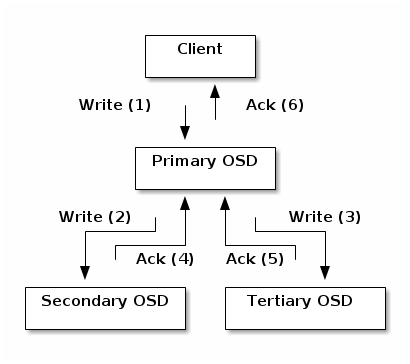
\includegraphics[scale=0.60]{replication.png}
	\caption{OSD Replication}
	\label{fig:osd_replication}
\end{figure}

With the ability to perform data replication, Ceph OSD Daemons relieve Ceph
clients from that duty, while ensuring high data availability and data safety.

\subsection{Dynamic Cluster Management}

In the section \ref{scal_and_high_avail}, we explained how Ceph uses CRUSH,
cluster awareness and intelligent daemons to scale and maintain high
availability. Key to Ceph’s design is the autonomous, self-healing, and
intelligent Ceph OSD Daemon. Let’s take a deeper look at how CRUSH works to
enable modern cloud storage infrastructures to place data, rebalance the
cluster and recover from faults dynamically.

\subsection{About Pools}
The Ceph storage system supports the notion of 'Pools', which are logical
partitions for storing objects.

Ceph Clients retrieve a Cluster Map(\ref{cluster_map}) from a Ceph Monitor, and
write objects to pools. The pool's size or number of replicas, the CRUSH
ruleset and the number of placement groups determine how Ceph will place the
data.

\begin{figure}[h]
	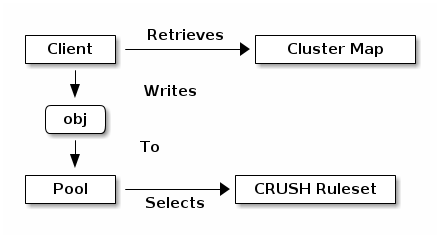
\includegraphics[scale=0.75]{pool_usage.png}
	\caption{Writing Data to Pools}
	\label{fig:pool_usage}
\end{figure}

Pools set at least the following parameters:

\begin{itemize}
	\item Ownership/Access to Objects
	\item The Number of Placement Groups, and
	\item The CRUSH Ruleset to Use
\end{itemize}

\subsection{Mapping PGs to OSDs}

Each pool has a number of placement groups. CRUSH maps PGs to OSDs dynamically.
When a Ceph Client stores objects, CRUSH will map each object to a placement
group.

Mapping objects to placement groups creates a layer of indirection between the
Ceph OSD Daemon and the Ceph Client. The Ceph Storage Cluster must be able to
grow (or shrink) and rebalance where it stores objects dynamically. If the Ceph
Client “knew” which Ceph OSD Daemon had which object, that would create a tight
coupling between the Ceph Client and the Ceph OSD Daemon. Instead, the CRUSH
algorithm maps each object to a placement group and then maps each placement
group to one or more Ceph OSD Daemons. This layer of indirection allows Ceph to
rebalance dynamically when new Ceph OSD Daemons and the underlying OSD devices
come online. The diagram(\ref{fig:pg_mapping}) depicts how CRUSH maps objects to
placement groups, and placement groups to OSDs.

\begin{figure}[h]
	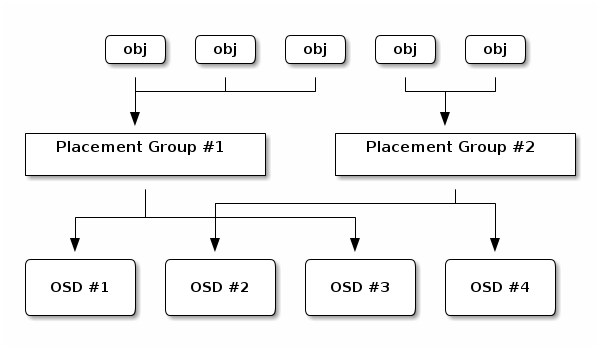
\includegraphics[scale=0.60]{pg_mapping.png}
	\caption{PG mapping}
	\label{fig:pg_mapping}
\end{figure}

With a copy of the cluster map and the CRUSH algorithm, the client can compute
exactly which OSD to use when reading or writing a particular object.

\subsection{Calculating PG IDs}

When a Ceph Client binds to a Ceph Monitor, it retrieves the latest copy of the
Cluster Map. With the cluster map, the client knows about all of the monitors,
OSDs, and metadata servers in the cluster. However, it doesn’t know anything
about object locations.

Object locations get computed.

The only input required by the client is the object ID and the pool. It’s
simple: Ceph stores data in named pools (e.g., ``liverpool''). When a client
wants to store a named object (e.g., ``john,'' ``paul,'' ``george,'' ``ringo'', etc.)
it calculates a placement group using the object name, a hash code, the number
of PGs in the pool and the pool name. Ceph clients use the following steps to
compute PG IDs.

\begin{enumerate}
	\item The client inputs the pool ID and the object ID. (e.g., pool =
		“liverpool” and object-id = “john”)
	\item Ceph takes the object ID and hashes it.
	\item Ceph calculates the hash modulo the number of PGs. (e.g., 58) to
		get a PG ID.
	\item Ceph gets the pool ID given the pool name (e.g., “liverpool” = 4)
	\item Ceph prepends the pool ID to the PG ID (e.g., 4.58).
\end{enumerate}

Computing object locations is much faster than performing object location query
over a chatty session. The CRUSH algorithm allows a client to compute where
objects should be stored, and enables the client to contact the primary OSD to
store or retrieve the objects.

\subsection{Peering and Sets}

In previous sections, we noted that Ceph OSD Daemons check each others
heartbeats and report back to the Ceph Monitor. Another thing Ceph OSD daemons
do is called ‘peering’, which is the process of bringing all of the OSDs that
store a Placement Group (PG) into agreement about the state of all of the
objects (and their metadata) in that PG. In fact, Ceph OSD Daemons Report
Peering Failure to the Ceph Monitors. Peering issues usually resolve
themselves; however, if the problem persists, you may need to refer to the
Troubleshooting Peering Failure section. \emph{Agreeing on the state does not mean
that the PGs have the latest contents.}

The Ceph Storage Cluster was designed to store at least two copies of an object
(i.e., size = 2), which is the minimum requirement for data safety. For high
availability, a Ceph Storage Cluster should store more than two copies of an
object (e.g., size = 3 and min size = 2) so that it can continue to run in a
degraded state while maintaining data safety.

Referring back to the diagram \ref{fig:osd_replication}, we do not
name the Ceph OSD Daemons specifically (e.g., osd.0, osd.1, etc.), but rather
refer to them as Primary, Secondary, and so forth. By convention, the Primary
is the first OSD in the Acting Set, and is responsible for coordinating the
peering process for each placement group where it acts as the Primary, and is
the ONLY OSD that that will accept client-initiated writes to objects for a
given placement group where it acts as the Primary.

When a series of OSDs are responsible for a placement group, that series of
OSDs, we refer to them as an Acting Set. An Acting Set may refer to the Ceph
OSD Daemons that are currently responsible for the placement group, or the Ceph
OSD Daemons that were responsible for a particular placement group as of some
epoch.

The Ceph OSD daemons that are part of an Acting Set may not always be up. When
an OSD in the Acting Set is up, it is part of the Up Set. The Up Set is an
important distinction, because Ceph can remap PGs to other Ceph OSD Daemons
when an OSD fails.

\emph{In an Acting Set for a PG containing osd.25, osd.32 and osd.61, the first
OSD, osd.25, is the Primary. If that OSD fails, the Secondary, osd.32,
becomes the Primary, and osd.25 will be removed from the Up Set.}

\end{document}
